\documentclass[12pt]{report}
\usepackage{styles/log-style}
\usepackage{setspace}  

\title{lab_report}
\author{Рамиль Титеев}
\date{September 2022}

\begin{document}
    \begin{titlepage}
        \begin{center}
            \large{Московский Aвиационный Институт}\\
            \large{(Национальный Исследовательский Университет)}\\
            \vspace{0.4in}
            \textbf{\LARGE{Факультет информационных технологий и прикладной математики}}\\
            \vspace{0.4in}
            \large{Кафедра вычислительной математики и программирования}\\
            \vspace{0.4in}
            \textbf{\LARGE{Лабораторная работa 8 по курсу ОOП:}}\\
            \textbf{\LARGE{основы программирования на языке С\#}}\\
        \end{center}
        \vspace{0.6in}
        \small{8. КОНКРЕТИЗАЦИЯ}\\
        \vfill
        \begin{flushleft}
                \large{ 
                    Работу выполнил:\\
                    М8О-205Б-21 \hspace{0.1in} 
                    Титеев Р.М. \hspace{0.3in}  
                    \tline{(\textit{подпись})}{\hspace{1in}} 
                    \hspace{0.3in} 
                    \tline{(\textit{вариант})}{\hspace{0.7in}}\\ 
                    Руководитель: \tline{(\textit{подпись})}{\hspace{1in}}/Кузнецова С.В. \\
                    Дата: \underline{\hspace{0.4in}} октября 2022\\
                }
        \end{flushleft}        
    \end{titlepage}

    \textbf{\large{Конкретизация}}\\
    \textbf{Текст программы}\\
    \begin{lstlisting}[language={[Sharp]C}]
using System;
using System.Collections.Generic;
using System.Linq;
using System.Text;
using System.Threading.Tasks;

namespace lab_2_1
{
    class A
    {
        private B b = new B();
        private C c = new C();
        public A() { }
        public void mA()
        {
            Console.WriteLine("method of A");
        }
        public B bA
        {
            get { Console.Write("get b ->"); return b; }
        }
        public C cA
        {
            get { Console.Write("get c ->"); return c; }
        }
    }

    class B
    {
        private D d = new D();
        public B() { }
        public void mB()
        {
            Console.WriteLine(" method of B");
        }
        public D dA
        {
            get { Console.Write("get d ->"); return d; }
        }
    }

    class C
    {
        private J j = new J();
        private E e = new E();
        public C()
        {
            this.c_val = 0;
        }
        public void mC()
        {
            Console.WriteLine(" method of C");
        }
        public E eA
        {
            get { Console.Write("get e ->"); return e; }
        }
        public J jA
        {
            get { Console.Write("get j ->"); return j; }
        }
        public int c_val { set; get; }
    }

    class D
    {
        public D() { }
        public void mD()
        {
            Console.WriteLine(" method of D");
        }
    }

    class E
    {
        private D d = new D();
        public E() { }
        public void mE()
        {
            Console.WriteLine(" method of E");
        }

        public D dA
        {
            get { Console.Write("get d ->"); return d; }
        }
    }

    class J
    {
        private K k = new K();
        public J() { }
        public void mJ()
        {
            Console.WriteLine(" method of J");
        }

        public K kA
        {
            get { Console.Write("get k ->"); return k; }
        }
    }
    class K
    {
        public K() { }
        public void mK()
        {
            Console.WriteLine(" method of K");
        }
    }
    internal class Program
    {
        static void Main(string[] args)
        {
            A a = new A();
            a.mA();
            a.bA.mB();
            a.cA.mC();

            a.bA.dA.mD();
            a.cA.jA.mJ();
            a.cA.eA.mE();

            a.cA.jA.kA.mK();

            Console.WriteLine($"a.cA.c_val: {a.cA.c_val}");
            a.cA.c_val = 15;
            Console.WriteLine($"a.cA.c_val: {a.cA.c_val}");

            Console.ReadKey();
        }
    }
}

\end{lstlisting}
    \vspace{0.4in}
    \newpage
    \textbf{Результат работы}\\
    \begin{center}
        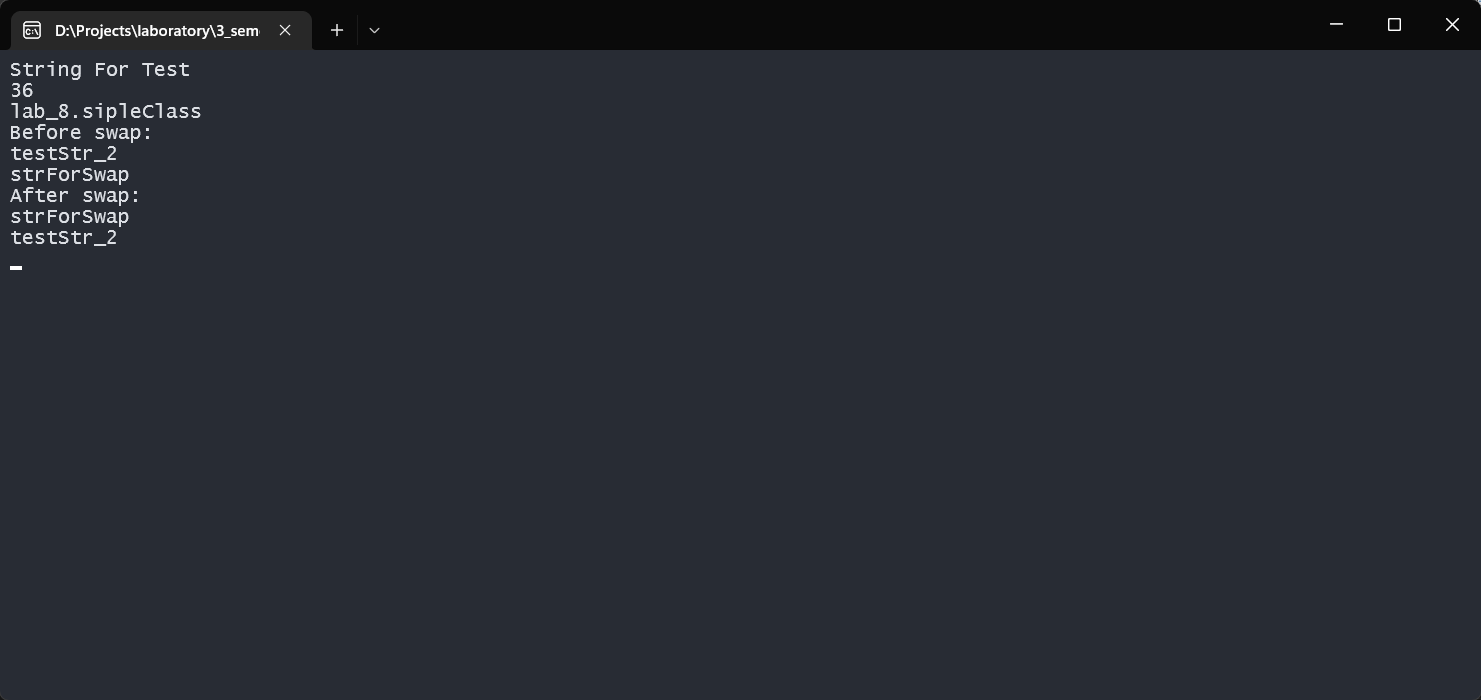
\includegraphics[scale=0.5]{formal/lab_8.png}\\
    \end{center}

    \textbf{Вывод}\\
    Конкретизация позволяет описывать классы и функции для работы с объектами, 
    типы которых заранее не определены. С каким(и) именно типам(и) придется работать 
    определяется в момент вызова – имя типа настраивает функцию или класс для работы.

\end{document}
